\documentclass[a4paper,11pt]{article}


\usepackage{alphabeta}
\usepackage{graphicx}

\usepackage[utf8x]{inputenc}

\usepackage{amsfonts , amssymb , amsmath}
\usepackage{float}
\usepackage{multirow}
\usepackage{amsmath}

\title{Αριθμητική Ανάλυση - 1η Εργασία}
\author{Ονοματεπώνυμο: Νικόλαος Ιλαρίδης \\ ΑΕΜ: 4524}
\date{\today}



\begin{document}
	\maketitle
	
	\section{Εισαγωγή}
	\begin{center}
		Τα προγραμματα για την εργασια εχουν υλοποιηθει με \textbf{python} και \textbf{matlab}. Σε ορισμενα σημεια της εργασιας εχει γινει χρηση γλωσσικου μοντελου "\textbf{chatGpt}" στα οποια και αναγραφεται σε σχολια στο εκαστοτε προγραμμα καθως υπαρχει και ο αντιστοιχος σχολιασμος στην περιγραφη της υλοποιησης μου.
	\end{center}
	\section{Πρώτη Ασκηση}
	\begin{center}
		\emph{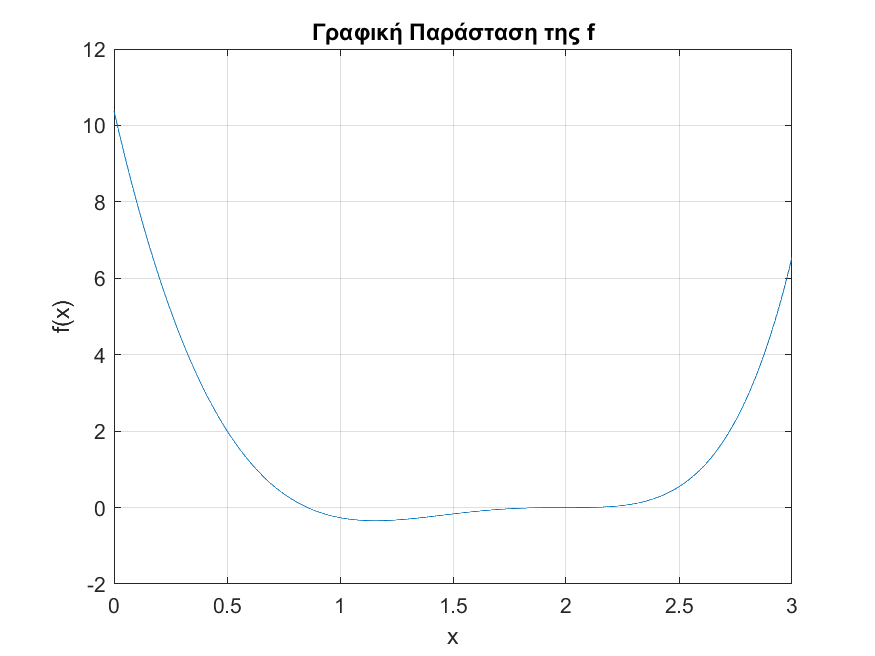
\includegraphics[scale=0.75]{ex1_graph.png}}
	\end{center}
	
\vspace{5cm}	
	\begin{enumerate}
			\item[\textbf{(α)}] \emph {\textbf{Μέθοδος Διχοτόμησης}}
	\end{enumerate}
	

	\begin{center}
		Στο αρχειο '\textbf{bisectionMethod.py}' που βρισκεται στον φακελο 'Ex1' υλοποιω την μεθοδο της διχοτομησης για τον υπολογισμο ριζων της δοθεισας συναρτησης 
	\end{center}
	
	\begin{center}
		Τα βηματα που ακολουθω ειναι τα εξης:
	\end{center}
	
	\begin{enumerate}
		\item {\emph{Aρχικοποιω την συναρτηση που μας ενδιαφερει. }}
		\item {\emph{Oριζω μια μεταβλητη mid η οποια ειναι το μεσο του τρεχοντος διαστηματος.}}
		\item {\emph{Κανω χρηση μιας while η οποια τερματιζει οταν η αποσταση των 2 ακρων ειναι μικροτερη του lim δηλαδη το αποδεκτο σφαλμα των 5 δεκαδικων ψηφιων.}}
		\item {\emph{Μεσα στον βροχο υπολογιζω καθε φορα το νεο mid και αυξανω τον μετρητη times χωριζοντας ετσι το μεγαλο διαστημα σε υποδιαστηματα μεχρι να προσεγγισω την ριζα της συναρτησης.}}
		\item {\emph{Επειδη ομως η συναρτηση στο διαστημα [0,3] εχει ομοσημες τιμες στα ακρα πρεπει να σπασω το διαστημα μου καθως η μεθοδος της διχοτομησης βασιζεται στο θεορημα Βolzano. Για αυτον τον λογο εκτυπωνω το αντιστοιχο μηνυμα και εκτελω τον αλγοριθμο στα διαστηματα [0,1] και [1.5,3]
		}}
	\end{enumerate}
	
\vspace{0.2cm}
	\begin{enumerate}
		\item[\textbf{(β)}] \emph {\textbf{Μεθοδος Newton-Raphson}}
	\end{enumerate}
	\begin{center}
		Στο αρχειο '\textbf{newtonRaphson.py}' που βρισκεται στον φακελο 'Ex1' υλοποιω την μεθοδο Newton Raphson για τον υπολογισμο ριζων της δοθεισας συναρτησης 
	\end{center}
		\begin{center}
		Τα βηματα που ακολουθω ειναι τα εξης:
	\end{center}
	
	\begin{enumerate}
		\item {\emph{Aρχικοποιω την συναρτηση f καθως και την πρωτη παραγωγο της \textbf{derivative1\_f}}}
		\item {\emph{Οριζω μια αρχικη εκτιμηση x0 }}
		\item {\emph{Χρησιμοποιω ενα βροχο while ο οποιος τερματιζει αν βρεθει η ριζα ή φτασει στον μεγιστο αριθμο επαναληψεων}}
		\item {\emph{Εντος της while υπολογιζω μια εκτιμιση της ριζας και ελεγχω αν η απολυτη τιμη της διαφορας της προηγουμενης και της νεας προσεγγισης ειναι μικροτερη του αποδεκτου σφαλματος}}
		\item {\emph{Αν δεν συγκλινει τοτε η νεα εκτιμηση x1 γινεται x0 και το i αυξανεται κατα 1}}		
	\end{enumerate}
	

	\begin{center}
		Επιπλεον αν καλεσουμε την συναρτηση '\textbf{newtonRaphson}' με ορισμα True στην δευτερη παραμετρο , παρατηρουμε οτι για την πρωτη ριζα το τετραγωνο της καθε προσεγγισης ειναι ισο με την προηγουμενη προσεγγιση αρα υπαρχει τετραγωνικη συγκλιση σε αντιθεση με την δευτερη . Αυτο ειναι αναμενομενο και απο την γραφικη παρασταση της f καθως στη δευτερη ριζα η καμπυλη εχει μικρη κλιση αρα και μικρη παραμετρο.  
	\end{center}
		
\vspace{1cm}
	\begin{enumerate}
		\item[\textbf{(γ)}] \emph {\textbf{Μεθοδος Τεμνουσας}}
	\end{enumerate}
	\begin{center}
		Στο αρχειο '\textbf{SecantMethod.py}' που βρισκεται στον φακελο 'Ex1' υλοποιω την μεθοδο Secant για τον υπολογισμο ριζων της δοθεισας συναρτησης 
	\end{center}
	\begin{center}
		Η μεθοδος Τεμνουσας απαιτει δυο αρχικες υποθεσεις και εκτελειται εως οτου ικανοποιηθουν καποιο απο τα 2 κρητιρια :  
	\end{center}
	\begin{enumerate}
		\item {\emph{Η απολυτη τιμη της συναρτησης (\textbf{abs(f(x1))}) ειναι μικροτερη απο την επιθυμητη ακριβεια (\textbf{tolerance})  }}
		\item {\emph{Εχει φτασει τον μεγιστο αριθμο επαναληψεων (\textbf{MAX})}}		
	\end{enumerate}
	\begin{center}
		Ωστοσο στην αποδοση της μεθοδου παιζει σημαντικο ρολο η επιλογη των αρχικων υποθεσεων , καθως αν οι υποθεσεις ειναι μακρια μεταξυ τους η συναρτηση μπορει να εχει λανθασμενο αποτελεσμα
	\end{center}
	
	\begin{enumerate}
		\item[\textbf{(δ)}] \emph {\textbf{Συγκριση Αποτελεσματων}}
	\end{enumerate}
	\begin{enumerate}
		\item[\text{1.}]  {\text{\textbf{Bisection Method}}
		\begin{enumerate}
			\item[\text{(a)}]{\text{Ριζα: 0.85715 Επαναληψεις: 18}}
			\item[\text{(b)}]{\text{Ριζα: 2.00000 Επαναληψεις: 17}}
		\end{enumerate}
		}
		\item[\text{2.}]  {\text{\textbf{Newton Raphson}}
			\begin{enumerate}
				\item[\text{(a)}]{\text{Ριζα: 0.85714 Επαναληψεις: 6}}
				\item[\text{(b)}]{\text{Ριζα: 2.00000 Επαναληψεις: 33}}
			\end{enumerate}
		}
		\item[\text{3.}]  {\text{\textbf{Secant Method}}
			\begin{enumerate}
				\item[\text{(a)}]{\text{Ριζα: 0.85714 Επαναληψεις: 7}}
				\item[\text{(b)}]{\text{Ριζα: 1.99368 Επαναληψεις: 14}}
			\end{enumerate}
		}
		
	\end{enumerate}
	\begin{center}
		Για την μεθοδο της διχοτομησης παρατηρουμε οτι στην πρωτη ριζα συγκλινει διακριτα πιο αργα απο τις αλλες 2 μεθοδους . Ομως στην δευτερη ριζα η μεθοδος διχοτομησης φαινεται να συγκλινει γρηγορα και με ακριβεια γεγονος που οφειλεται στις τιμες της f κοντα απο την ριζα οι οποιες ειναι αρκετα κοντα στο 0. Απο την αλλη πλευρα οι αλλες 2 μεθοδοι στην πρωτη ριζα συγκλινουν παρομοια ενω στην δευτερη ριζα η Secant φαινεται να ξεχωριζει , ωστοσο οφειλεται στις αρχικες υποθεσεις που δινουμε στην καθε μεθοδο
	\end{center}
	
	\section{Δεύτερη Ασκηση}
	
	\begin{enumerate}
		\item[\textbf{(α)}] \emph {\textbf{Τροποποιημενη Μέθοδος Διχοτόμησης}}
	\end{enumerate}
	\begin{center}
		Η διαφορα της τροποποιημενης μεθοδου ειναι η χρηση ενος τυχαιου αριθμου σε αντιθεση με την κλασικη που αρχικοποιουμε με το μεσο του διαστηματος.
	\end{center}
	
	\begin{enumerate}
		\item[\textbf{(β)}] \emph {\textbf{Τροποποιημενη Newton Raphson}}
	\end{enumerate}
	\begin{center}
		Η μονη διαφορα της τροποποιημενης Newton Raphson με την γνησια ειναι η χρηση της δευτερης παραγωγου για την εκτιμηση της ριζας . 
	\end{center}
	
	\begin{enumerate}
		\item[\textbf{(γ)}] \emph {\textbf{Τροποποιημενη Μέθοδος Τέμνουσας}}
	\end{enumerate}
	\begin{center}
		Η διαφορα της τροποποιημενης μεθοδου ειναι η χρηση 3 αρχικων σημειων σε αντιθεση με την γνησια που χρειαζεται μονο 2 καθως και ο νεος τυπος βαση του οποιου γινεται η εκτιμηση 
	\end{center}
	
	
	\begin{enumerate}
		\item[\textbf{(δ)}] \emph {\textbf{Συγκριση Αποτελεσματων}}
	\end{enumerate}
	\begin{enumerate}
		\item[\text{1.}]  {\text{\textbf{mod Bisection Method}}
			\begin{enumerate}
				\item[\text{(a)}]{\text{Ριζα: -1.38212 Επαναληψεις: 20}}
				\item[\text{(b)}]{\text{Ριζα: notFound Επαναληψεις: -}}
				\item[\text{(c)}]{\text{Ριζα: 0.20518 Επαναληψεις: 20}}
				\item[\text{(d)}]{\text{Ριζα: 0.50008 Επαναληψεις: 20}}
				\item[\text{(e)}]{\text{Ριζα: 1.17611 Επαναληψεις: 20}}
			\end{enumerate}
		}
		\item[\text{2.}]  {\text{\textbf{mod Newton Raphson}}
			\begin{enumerate}
				\item[\text{(a)}]{\text{Ριζα: -1.38130 Επαναληψεις: 5}}
				\item[\text{(b)}]{\text{Ριζα: -0.66667 Επαναληψεις: 14}}
				\item[\text{(c)}]{\text{Ριζα: 0.20518 Επαναληψεις: 4}}
				\item[\text{(d)}]{\text{Ριζα: 0.50000 Επαναληψεις: 5}}
				\item[\text{(e)}]{\text{Ριζα: 1.17612 Επαναληψεις: 5}}
			\end{enumerate}
		}
		\item[\text{3.}]  {\text{\textbf{mod Secant Method}}
			\begin{enumerate}
				\item[\text{(a)}]{\text{Ριζα: -1.38132 Επαναληψεις: 8}}
				\item[\text{(b)}]{\text{Ριζα: -0.66667 Επαναληψεις: 23}}
				\item[\text{(c)}]{\text{Ριζα: 0.20518 Επαναληψεις: 4}}
				\item[\text{(d)}]{\text{Ριζα: 0.50000 Επαναληψεις: 6}}
				\item[\text{(e)}]{\text{Ριζα: 1.17609 Επαναληψεις: 5}}
			\end{enumerate}
		}
		
		
	\end{enumerate}
		\begin{center}
			Παρατηρουμε οτι με την μεθοδο Διχοτομησης δεν μπορουμε να βρουμε την δευτερη ριζα . Αυτο οφειλεται στο γεγονος οτι η συναρτηση γυρω απο αυτη την ριζα δεν αποκταει θετικες τιμες γεγονος που οδηγει σε αποτυχια λογω του Θ.Bolzano. Επισης ειναι διακριτο πως η Μεθοδος Διχοτομησης ειναι σημαντικα πιο αργη απο τις υπολοιπες , οι οποιες εμφανιζουν πολυ παρομοα αποτελεσματα τοσο στις ριζες οσο και στις επαναληψεις
		\end{center}
		
	\begin{enumerate}
		\item[\textbf{(ε)}] \emph {\textbf{Διαφορα  Αποτελεσματων}}
	\end{enumerate}
	\begin{center}
		Εκτελώντας τον αλγοριθμο modBisection 20 φορες διαπιστωνουμε οτι η τροποποιημενη μεθοδος διχοτομησης εμφανιζει διαφορετικο αποτελεσμα επαναληψεων γεγονος που οφειλεται στην χρηση τυχαιου αριθμου .
	\end{center}
	\begin{enumerate}
		\item[\textbf{(στ)}] \emph {\textbf{Διαφορα  Χρονου Εκτελεσης}}
	\end{enumerate}
	\begin{center}
		Υπολογιζοντας τον συνολικο χρονο εκτελεσης του καθε αλγοριθμου διαπιστωστα οτι οι τροποποιημενες μεθοδοι κατα μεσο ορο συγκλινουν πιο γρηγορα απο τις γνησιες.
	\end{center}
	\begin{enumerate}
		\item[\text{(a)}] {\text{Bisection : 0.000459 }}
		\item[\text{(b)}] {\text{Newton Raphson : 0.000656 }}
		\item[\text{(c)}] {\text{Secant : 0.00011 }}
	\end{enumerate}
\vspace{0,5cm}
	\begin{enumerate}
		\item[\text{(a)}] {\text{mod Bisection : 0.00037 }}
		\item[\text{(b)}] {\text{mod Newton Raphson : 0.00133 }}
		\item[\text{(c)}] {\text{mod Secant : 0.00003 }}
	\end{enumerate}
\vspace{4cm}
	\section{Τρίτη Ασκηση}
	
	\begin{enumerate}
		\item[\textbf{(α)}] \emph {\textbf{PA = LU}}
	\end{enumerate}
	\begin{center}
		Στο προγραμμα \underline{PA\_LU.py} βρισκω την λυση του συστηματος \textbf{Ax=b} με την μεθοδο \textbf{PA=LU}. Πιο συγκεκριμενα αρχικα πραγματοποιω διασπαση LU στον πινακα Α με την μεθοδο gauss δημιουργοντας ετσι ενα ανω και ενα κατω τριγωνικο πινακα. Στην συνεχεια λυνω το συστημα \textbf{Ly = b} ή αλλιως κανω Forward Substitution και επειτα λυνω το συστημα \textbf{Ux=y} ή αλλιως Backward Substitution . Καταυτον τον τροπο εχω λυσει το αρχικο συστημα \textbf{Ax=b}
	\end{center}
	\begin{enumerate}
		\item[\textbf{(β)}] \emph {\textbf{Cholesky}}
	\end{enumerate}
	\begin{center}
		Ο αλγοριθμος \textbf{Cholesky} λαμβανει ενα πινακα συμμετρικο και θετικα ορισμενο και επιστρεφει ενα κατω τριγωνικο πινακα L καθως και τον αναστροφο του. Ωστοσο η εκφωνηση ζηταει μονο τον πινακα L . Η μεθοδος Cholesky μοιζει με την αναλυση \textbf{PA=LU} ωστοσο ειναι αρκετα πιο αποδοτικος. 
	\end{center}
	\begin{center}
		Στην υλοποιηση μου εχω κανει χρηση γλωσσικου μοντελου '\textbf{chatGpt}' . Στο αρχειο \textbf{cholesky.py} εχω γραψει σε σχολια τα σημεια που εχω χρησιμοποιησει το γλωσσικο μοντελο καθως και τον κωδικα μου πριν γινει η χρηση. Μαλιστα ο δικος μου κωδικας ειχε προβλημα στον υπολογισμο της μεταβλητης Sum η οποια χρησιμοποιοταν στον τυπο υπολογισμου του L
	\end{center}
	\begin{enumerate}
		\item[\textbf{γ)}] \emph {\textbf{Gauss-Seidel}}
	\end{enumerate}
	\begin{center}
		Η μεθοδος \textbf{Gauss-Seidel} χρησιμοποιειται για την επιλυση γραμμικων συστηματων . Πιο συγκεκριμενα η συναρτηση που εχω υλοποιησει δεχεται εισοδο ενα πινακα Α και ενα διανυσμα b και επιστρεφει το διανυσμα x το οποιο υπολογιζεται με βαση τον τυπο που δινεται στην εκφωνηση . Η διαδικασια σταματαει οταν η διαφορα των 2 διαδοχικων επαναληψεων ειναι μικροτερη του αποδεκτου σφαλματος ή αν εκτελεστει ο βροχος πανω απο τις μεγιστες επιθυμητες επαναληψεις
	\end{center}
	\section{Τέταρτη Ασκηση}
	\begin{enumerate}
		\item[\textbf{4.1)}] \emph {\textbf{Αποδειξη Στοχαστικου}}
	\end{enumerate}
	\begin{center}
		Για να ειναι ο πινακας \textbf{G} στοχαστικος θα πρεπει το αθροισμα καθε στηλης του πινακα να ισουται με 1. Ετσι στο προγραμμα \textbf{Ex4.py} υπολογιζω το αθροισμα καθε στηλης του πινακα το οποιο ειναι ισο με 1 , αρα οντως ειναι στοχαστικος . 
	\end{center}
	\begin{enumerate}
		\item[\textbf{4.2)}] \emph {\textbf{Ιδιοδιανυσμα Μεγιστης Ιδιοτιμης}}
	\end{enumerate}
	\begin{center}
		Ο πινακας Google υπολογιζεται απο την συναρτηση \textbf{calc\_G(A,q)}, η οποια αρχικοποιει τον πινακα με 0 και στην συνεχεια με βαση τον τυπο που δινεται υπολογιζει τις τιμες του . 
	\end{center}
	\begin{center}
		Η ευρεση του ιδιοδιανυσματος με την μεγαλυτερη ιδιοτιμη γινεται με την μεθοδο δυναμεως (\textbf{Power Method}) ακολουθοντας τα εξης βηματα : 
	\end{center}
	\begin{enumerate}
		\item[\text{(1)}] {\text{Δημιουργω ενα τυχαιο διανυσμα x}}
		\item[\text{(2)}] {\text{Το αναλυω σε συνιστωσες x0 x1}}
		\item[\text{(3)}] {\text{Ελεγχω αν πληρουνται τα κρητιρα συγκλισης }}
		\item[\text{(4)}] {\text{Ενημερωνω καταλληλα το ιδιοδιανυσμα}}
		\item[\text{(5)}] {\text{Κανονικοποιω}}
	\end{enumerate}
	
	\begin{enumerate}
		\item[\textbf{4.3)}] \emph {\textbf{Νεος Πινακας G}}
	\end{enumerate}
	\begin{center}
		Για το συγκεκριμενο ερωτημα επελεξα να βελτιωσω τον βαθμο σημαντικοτητας της Σελιδας 15.Ετσι δημιουργησα 4 νεες ακμες :
		\begin{enumerate}
			\item[\text{(1)}] {\text{12-15}}
			\item[\text{(2)}] {\text{8-15}}
			\item[\text{(3)}] {\text{15-11}}
			\item[\text{(4)}] {\text{10-15}}
		\end{enumerate}
		Ετσι υπολογιζοντας την σημαντικοτητα της Σελιδας 15 πριν και μετα την αλλαγη παρατηρουμε οτι αυξηθηκε απο 1.2125 σε 2.1333333333
	\end{center}
		\begin{enumerate}
		\item[\textbf{4.4)}] \emph {\textbf{Αλλαγη q}}
	\end{enumerate}
	\begin{center}
		Αλλαζοντας την πιθανοτητα q σε 0.02 και 0.6 διακρινουμε οτι οσο μεγαλυτερη τιμη εχει η πιθανοτητα q τοσο πιο 'αχρηστο' γινεται το pagerank καθως ολες οι τιμες ειναι πιο κοντα μεταξυ τους .
	\end{center}
	\begin{center}
		Ο σκοπος της πιθανοτητας q ειναι να προσομοιωνει την συμπεριφορα του χρηστη που μεταπηδαει τυχαια απο μια σελιδα σε μια αλλη .
	\end{center}
	
	\begin{enumerate}
		\item[\textbf{4.5)}] \emph {\textbf{Αλλαγη στον πινακα γειτνιασης}}
	\end{enumerate}
	\begin{center}
			Μετα την αλλαγη των κελιων [8,11] και [12,11] σε 3 παρατηρουμε μια αυξηση στην συμαντικοτητα της Σελιδας 11. Ετσι μπορουμε να πουμε πως η στρατηγικη αυτη δουλευει καθως υπηρξε σημαντικη αλλαγη στο pagerank
	\end{center}
	\begin{enumerate}
		\item[\textbf{4.6)}] \emph {\textbf{Διαγραφη Σελιδας 10}}
	\end{enumerate}
	
	
	\begin{enumerate}
		\item[\text{(1)}] {Page 1: 0.0268236 - Page 1 after: 0.0470966}
		\item[\text{(2)}] {Page 2: 0.0298616 - Page 2 after: 0.0409113}
		\item[\text{(3)}] {Page 3: 0.0298613 - Page 3 after: 0.0359354}
		\item[\text{(4)}] {Page 4: 0.0268228 - Page 4 after: 0.0320696}
		\item[\text{(5)}] {Page 5: 0.0395888 - Page 5 after: 0.0428002}
		\item[\text{(6)}] {Page 6: 0.0395886 - Page 6 after: 0.0413910}
		\item[\text{(7)}] {Page 7: 0.0395877 - Page 7 after: 0.0516587}
		\item[\text{(8)}] {Page 8: 0.0395876 - Page 8 after: 0.0502495}
		\item[\text{(9)}] {Page 9: 0.0745681 - Page 9 after: 0.0482228}
		\item[\text{(10)}] {Page 10: 0.1063182 - Page 10 after: -}
		\item[\text{(11)}] {Page 11: 0.0745663 - Page 11 after: 0.1709634}
		\item[\text{(12)}] {Page 12: 0.1063163 - Page 12 after: 0.1035985}
		\item[\text{(13)}] {Page 13: 0.1250889 - Page 13 after: 0.0411622}
		\item[\text{(14)}] {Page 14: 0.1163333 - Page 14 after: 0.1074622}
		\item[\text{(15)}] {Page 15: 0.1250867 - Page 15 after: 0.1864787}
	\end{enumerate}
	
	\begin{center}
		Παρατηροντας τις αλλαγες διακρινουμε μια μεγαλη πτωση στην τιμη της Σελιδας 13 . Αυτο συμβαινει καθως ηταν η μοναδικη ακμη με αρχη την Σελιδα 10 και εφοσον η Σελιδα 10 ειχε υψηλη επισκεψιμοτητα , ειναι αναμενομενη η πτωση της. 
	\end{center}
	
	
\end{document}